\documentclass[a4paper,11pt]{article}
\usepackage{f420}

\captionsetup{width=0.8\textwidth}

\begin{document}

\section{\bf Range-деревья}

\emph{Range-дерево (дерево параллелепипедов)}~— структура данных, позволяющая
хранить \(n\)~то\-чек \(p_1, p_2, \ldots, p_n \in \br^d\) и отвечать на
запросы вида «сколько точек \(p_i\) находится в параллелепипеде
\([x^1_1, x^1_2] \times \ldots \times [x^d_1, x^d_2]\)»
за время \(O (\log^{d-1} n)\); при этом построение структуры данных
для \(n\) точек занимает время \(O (n \cdot \log^{d-1} n)\).

При \(d \ge 2\) \(d\)-мерное дерево параллелепипедов устроено следующим
образом: это дерево отрезков для множества всех точек, упорядоченного по
первой координате, в каждой вершине которого хранится,
для множества всех точек \(p_i\) в листьях–потомках данной вершины,
\begin{itemize}
  \item их количество;
  \item наибольшее и наименьшее значение их первой координаты;
  \item \(d-1\)-мерное дерево параллелепипедов по оставшимся \(d-1\)
    координатам, кроме первой.
\end{itemize}

Дерево параллелепипедов размерности \(d-1\), построенное в данной
вершине \(d\)-мерного дерева для множества точек в её поддереве,
называется \emph{ассоциированной структурой},
см.~рисунок~\ref{fig:range-tree}.

\begin{figure}[h] \centering
  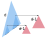
\includegraphics{img/range-tree}
  \caption{Ассоциированные структуры: в каждом внутреннем узле
    \(d\)-мерного дерева параллелепипедов~— \(d-1\)-мерное
    дерево, построенное для множества всех точек \(p_i\) под данным узлом}
  \label{fig:range-tree}
\end{figure}

Так как \(d\)-мерное дерево по сути \emph{состоит} из \(d-1\)-мерных,
то понимать, какое время требуется на построение и на запрос,
мы будем индукцией по размерности. Только \emph{базой индукции}
будет случай \(d = 2\): для двумерного дерева мы покажем, как его
можно нетривиально ускорить.

\begin{theorem}
  Пусть \(d \ge 3\); запрос к \(d\)-мерному дереву параллелепипедов
  сводится к \(\log n\) запросам к \(d-1\)-мерным деревьям.
\end{theorem}

\begin{proof}
Сначала вспомним, как устроен запрос к одномерному дереву
отрезков~— а устроен он следующим образом. Будем рекурсивно
спускаться из корня, и в текущей вершине для каждого из двух детей:
\begin{itemize}
  \item если отрезок, накрываемый им, не пересекает диапазон
    из запроса, — не вызываемся от этого ребёнка,
  \item если отрезок, накрываемый им, полностью содержится в диапазоне
    из запроса, — прибавляем к ответу количество точек, находящихся
    в листьях под этим ребёнком (это количество хранится
    непосредственно в нём);
  \item если отрезок, накрываемый им, пересекается с диапазоном
    из запроса, — вызываемся от него рекурсивно.
\end{itemize}

В общем, дерево отрезков в точности накрывает диапазон из запроса
поддеревьями \(\log n\) своих узлов, и ответ на запрос~— сумма
хранящихся в этих узлах количеств точек в листьях их поддерева.

Пусть теперь мы отвечаем на \(d\)-мерный запрос
\([x^1_1, x^1_2] \times \ldots \times [x^d_1, x^d_2]\).
Наше дерево параллелепипедов~— оно же дерево отрезков по первой
координате. Потому мы можем, как описано выше, накрыть множество
точек \(p_i\), первая координата которых лежит в отрезке
\([x^1_1, x^1_2]\), \(\log n\) вершинами дерева.

После этого останется из множеств точек \(p_i\) под каждой
из этих вершин отфильтровать те, оставшиеся координаты которых
лежат в интересующих нас диапазонах. Это можно сделать
как раз запросами к \(d-1\)-мерным деревьям.
\end{proof}

\begin{theorem}
  Пусть \(d \ge 3\). Если \(d-1\)-мерное дерево отрезков
  для \(n\) точек строится за время \(O (n \cdot \log^{d-2} n)\),
  то \(d\)-мерное дерево отрезков для \(n\) точек строится
  за время \(O (n \cdot \log^{d-1} n)\).
\end{theorem}

\begin{proof}  \begin{multline*}
  T(n)\ =\ 2 \cdot T \lr*{\frac n 2} + O (n \cdot \log^{d-2} n)\ =\ 
  \sum_{k = 0}^{\log n} 2^k \cdot \frac{n}{2^k} \cdot
    \log^{d-2} \lr*{\frac{n}{2^k}}\ = \\
  =\ n \cdot \lr*{\log^{d-2} n + \lr*{\log^{d-2} n}
    + \ldots + 1^{d-2}}
  \ =\ n \cdot \log^{d-1} n.
\end{multline*}  \end{proof}

\begin{theorem}
  Двумерное дерево параллелепипедов можно построить за время
  \(O (n \cdot \log n)\), а отвечать на запросы к нему~—
  за время \(O (\log n)\).
\end{theorem}

\begin{proof}
  То, что описано далее, гуглить/искать в [de Berg, van Kreveld et al.]
  по ключевым словам \emph{``fractional cascading''}.
  Для быстрого построения сначала упорядочим все точки по
  \emph{второй} координате, и в корне будем хранить \emph{массив}
  из всех точек (вместо одномерного дерева отрезков на них).
  
  Напомним, что в упорядоченном массиве тоже можно отвечать на запросы
  о количестве точек в диапазоне за \(\log n\): два двоичных поиска
  по краям диапазона, а затем разность индексов. А также в каждой вершине
  разбить множество точек на две половины по первой координате, найдя
  медиану по этой координате, можно за линейное время.
  
  (ссылки в массивы в детях)
\end{proof}

\end{document}
